%-------------------------------------------------------------------------------
\section{Background}
%------------------------------------------------------------------------------

This section presents the necessary background to facilitate the discussion for the rest of the paper, 
including a primer on large language model~(LLM) inference~(\S\ref{sec:llm}), 
the need to maintain latency SLOs during LLM inference~(\S\ref{sec:slo}), 
and memory offloading techniques for LLM~(\S\ref{sec:offloading}).

\subsection{A Primer on LLM Inference}
\label{sec:llm}
%
Large language models (LLMs), a new class of deep learning models, have demonstrated great success in various domains, 
such as data analysis~\cite{dataanalyse1, dataanalyse2, dataanalyse3},  
language translation~\cite{translation1, translation2, translation3}, 
content generation~\cite{content1, content2, content3}, and 
code development~\cite{code1, code2, code3, code4}. 
%
Such success is due to the fact that LLM can easily generalize across different 
tasks and efficiently process large amounts of unstructured data~\cite{Unstructured1}. 
%

During inference, an LLM takes as input a sequence of tokens~(\,  e.g., typically an English word), which is called a prompt. 
%
The sequence length denotes the number of tokens in a prompt. 
%
In addition, to maximize LLM inference performance, a common approach is to batch multiple prompts together to allow the GPU to process them simultaneously. 
%
The batch size is the number of prompts in a batch. 
%
The output of an LLM, called an output sequence, is also a sequence of tokens. 
%

This paper focuses on decoder-only LLMs, such as GPT~\cite{gpt}, LLaMA~\cite{llama}, and OPT~\cite{opt}, which are arguably the most common type of LLMs. 
%
These models are based on the Transformer~\cite{transformer} architecture, 
consisting of multiple decoder layers~(layers afterwards).  
%
Each layer has the same structure with the same number of matrices, with each corresponding matrix having the same dimensions. 
%
The only difference is the values of the elements within each matrix.

%
The computation during LLM inference is conducted in a layer-by-layer fashion; 
% 
LLM performs computation on one layer, updates the relevant state, and 
then moves to the next layer. 
%
Each layer performs the same set of operations, which involve attention computations to capture dependencies between tokens and MLP computations to transform and refine the representations. 



%

\PN{Prefill and Decoding.}
%
LLM inference consists of two phases: prefill and decoding.
%
During prefill, an LLM traverses each layer to generate the first token in the output sequence by processing all the tokens in the input sequence.
%
During decoding, the model generates the rest of the tokens iteratively. 
% 
In the first iteration, the model uses the token generated by the prefill phase
to produce the next token in the output sequence. 
%
Afterwards, the output token generated in the previous iteration 
is used as the input for the next iteration. 
%
The process stops when reaching a word limit or seeing a set of predefined end tokens or end patterns.
%

Critically, the prefill and decoding exhibit different characteristics.
%
The prefill phase is computation-intensive since it involves processing all the tokens in an input sequence.
%
The decoding phase is memory-intensive and only needs to process the token generated in the previous iteration. 
%


\subsection{LLM Inference with SLO requirements}
\label{sec:slo}
%
As discussed earlier, due to their powerfulness, LLMs are used for various tasks. 
%
Some of these tasks have a long serving time, on the order of a few hours, 
and do 
not require real-time interactions with human users. 
%
Examples include summarizing or translating large text corpora~\cite{hjx1, hjx2, hjx3}, 
bulk content generation~\cite{hjx4}, or offline analytics~\cite{hjx5, hjx6}. 
%

%
On the other hand, lots of LLM tasks, such as chatbots~\cite{chatbot1, chatbot2} and virtual assistants~\cite{virtualassist}, involve frequent interactions with human users.  
%
Thus, these tasks must be highly responsive and are often associated with  stringent latency service level objectives~(SLOs) that must be met since 
failing to do so incurs a severe economic loss.
%
For example, with production chatbot services, one latency SLO is that each token must be generated within hundreds of milliseconds to ensure timely feedback that aligns with human reading speeds~\cite{humanspeed}. 
%
Failing to meet the SLO would cause the users to experience delays and thus be more likely to switch to competing services. 


This paper targets two common latency SLOs: (1) Time to First Token~(TTFT)~(\ie, the amout of time to generate the first token of 
a response); 
%
and (2) Time Per Output Token~(TPOT)~(\ie, the average amount of time to 
produce the rest of the token, excluding the first one). 
%
TTFT and TPOT are used for SLOs of the prefill and decoding phases, respectively. 

\subsection{Offloading LLM to Host Memory}
\label{sec:offloading}
%

\begin{figure}[t]
    \centering
    \resizebox{0.65\columnwidth}{!}{%
        % This file was created with tikzplotlib v0.10.1.
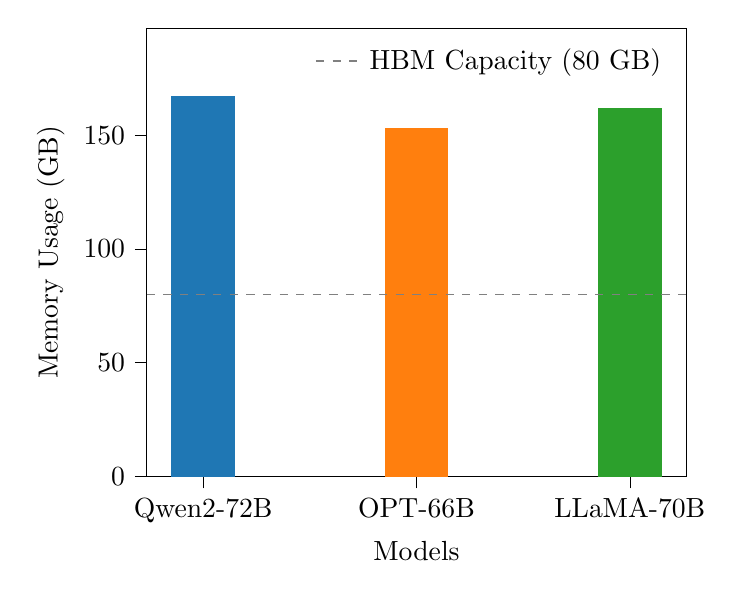
\begin{tikzpicture}

  \definecolor{darkgray176}{RGB}{176,176,176}
  \definecolor{darkorange25512714}{RGB}{255,127,14}
  \definecolor{forestgreen4416044}{RGB}{44,160,44}
  \definecolor{gray}{RGB}{128,128,128}
  \definecolor{steelblue31119180}{RGB}{31,119,180}
  
  \begin{axis}[
  legend cell align={left},
  legend style={fill opacity=0.8, draw opacity=1, text opacity=1, draw=none},
  tick align=outside,
  tick pos=left,
  x grid style={darkgray176},
  xlabel={Models},
  xmin=-0.265, xmax=2.265,
  xtick style={color=black},
  xtick={0,1,2},
  xticklabels={Qwen2-72B,OPT-66B,LLaMA-70B},
  y grid style={darkgray176},
  ylabel={Memory Usage (GB)},
  ymin=0, ymax=197,
  ytick style={color=black}
  ]
  \draw[draw=none,fill=steelblue31119180] (axis cs:-0.15,0) rectangle (axis cs:0.15,167);
  \draw[draw=none,fill=darkorange25512714] (axis cs:0.85,0) rectangle (axis cs:1.15,153);
  \draw[draw=none,fill=forestgreen4416044] (axis cs:1.85,0) rectangle (axis cs:2.15,162);
  \addplot [semithick, gray, dashed]
  table {%
  -0.265 80
  2.265 80
  };
  \addlegendentry{HBM Capacity (80 GB)}
  \end{axis}
  
  \end{tikzpicture}
   % 插入 TikZ 图
 }
    \caption{Memory demands of modern LLMs using float16 precision, with input sequences of 2,048 tokens. 
 The grey dashed line represents the GPU memory capacity (80GB) of the NVIDIA A100.}
    \label{fig:memoryuse}
\end{figure}


Modern LLMs often have tens to hundreds of billions of parameters with long prompt lengths. 
%
As a result, these models require hundreds of gigabytes of memory to handle daily requests, as shown in Figure~\ref{fig:memoryuse}
%
This demand far exceeds the capacity of even cutting-edge GPUs like the NVIDIA A100~\cite{A100}, which only equips 80GB of memory.
%

To address the growing memory demands of LLMs, a promising approach~\cite{lorazerooffload} 
is to offload part of the model state to host memory, which is traditionally used by CPUs. 
%
The offloaded state is transferred back to the GPU as needed. 
%
Offloading effectively reduces GPU memory usage, thereby achieving various benefits, including 1) enabling the deployment of powerful models that exceed GPU memory capacity, 2) allowing for the generation of longer output sequences, and 3) supporting larger inputs with greater batch sizes and/or input sequences. 

%
This offloading is effective because host memory is inherently larger than GPU memory. 
%
Modern servers often have several terabytes of host memory, while 
the memory of modern GPUs is often only a few tens of gigabytes. 
%
The orders-of-magnitude difference is due to 1) GPU memory, built using high-speed HBM and GDDR technologies, is significantly more expensive than the DDR SDRAM used in host memory, and 2) extending GPU memory is more challenging than host memory due to constraints on power consumption and heat dissipation. 

